\chapter{Simulation-based comparison of solar powered power plants}
To compare CSP and PV technologies, a simulated case study was performed on the basis of a CR system and PTC system. 
%Special attention was paid in this comparison for a high run time of the system during the day and the covering of a prescribed demand curve.
Specific attention was given to maximizing daytime operation and meeting the demand curve. 
% For this comparison the PV system was expanded with an electrical energy storage.
The photovoltaic system was extended with battery storage. 
% For the simulation an battery storage was selected.
% The dimension of the stored energy in this simulation went much beyond the actual technical capacity of individual electrical storage units and reaches more than one-sixt of the actual world battery storage capacity \SI{690}{GW} \cite{IEA2015}.
The storage capacity allocated for the simulation considerably exceeds the real capacity of electrical storage units currently available and is more than one-sixth the globally installed battery storage capacity of \SI{690}{GW}.\cite{IEA2015}
 %Therefor must be said at this point that this is a theoretical comparison from the viewpoint of the PV, in particular for this plant and storage scale.
Due to the scale and particularly with respect to the photovoltaic plant, the comparison is theoretical in nature.
\pagebreak
\section{General assumptions}
With the aim of producing quantifiable and comparable results, the different solar supplied power plants will be simulated under different input  parameters. After that, selected comparable output parameters will be analyzed, evaluated and rated.

The plant technologies selected for comparison are: 
\begin{itemize}
\item CSP molten salt central receiver with thermal energy storage
\item CSP synthetic oil parabolic trough with thermal energy storage
\item PV fixed elevated flat plate collectors with adapted electrical energy storage
\end{itemize}
The PV plant has been extended with a lithium-ion battery storage for the simulation, while the thermal energy storage of the CSP plant uses molten salt technology.
%All power plants got laid out for a maximum power output of \SI{100}{MW}$_{el}$.
All plants were laid out for a maximum power output of \SI{100}{\mega\wattel}.
% For the comparison the power plants are forced to cover a selected load scenario.
The plants are driven to match a selected load scenario.
% In order to find an individual suitable power plant design to cover the scheduled output of the scenario, different layout conditions, using various storage and collecting field sizes, was tried.
In order to find an appropriate power plant design to match the load of the scenario, different layout parameters, using various storage and collecting field sizes, were tested.
% The scenario and there goals are discussed and defined in Section~\ref{Overall simulated configuration}. The location and related weather data is defined in Section~\ref{Location and weather data}.
The scenario and requirements are defined and discussed in Section~\ref{Overall simulated configuration}. The location and related weather data are described in Section~\ref{Location and weather data}.
%The solar power plants are implemented and simulated in NREL’s System Advisor Model (SAM) version SAM 2015.6.30 r3 for OS X \cite{NREL2015}.
The solar power plants are implemented and simulated in NREL’s System Advisor Model (SAM) version SAM 2015.6.30 r3 for OS X \cite{NREL2015}. 
% SAM is designed to simulate performance and financial models of different types of renewable energies. For the simulation the performance part of the software was used. The financial analysis was made separately. 
SAM is designed to simulate performance and financial models of different types of renewable energy. For this simulation, only the performance component was used. The financial analysis was done separately. 

The financial parameters and the resulting levelized cost of electricity (LCOE) are calculated separately for all power plants in Microsoft Excel 2011 (vers. 14.5.7) for Mac, using a simplified method which is documented in Appendix~\ref{ChapterLCOE} on page \pageref{ChapterLCOE} using a lifetime of \SI{25}{years} for each plant.

\subsection{Scenario of simulations} \label{Overall simulated configuration}
%Power plants are forced to supply the system load/demand.
A hard requirement is that plants meet the full electrical demand in the system. Figure~\ref{LoadScenarios} shows the daily average system load/demand in South Africa for the winter and summer period.
% The profiles from both load shapes rises at approx 7:00 in the morning and has there peak demand at 20:00 during the summer period.
Both profiles feature a sharp rise at approx 7:00 and have their peak demand at 20:00 during the summer period.
In winter, there is an initial peak at 9:00 and a second at 19:00.
%In order to supply this system load the simulated solar power plants are forced to generate full power output of \SI{100}{MW} from 7:00 to 22:00. When the system demand comes down during the night also the power plants reduce there output from 22:00 to 7:00 to \SI{50}{MW}. The scenario is called "night-reduction".
In order to match this system load, the simulated solar power plants must operate at full power output of \SI{100}{MW} from 7:00 to 22:00. When the system demand drops during the night, the plants reduce there output from 22:00 to 7:00 to \SI{50}{MW}. The scenario is called "night reduction".
\begin{figure}[htbp]  
\centering
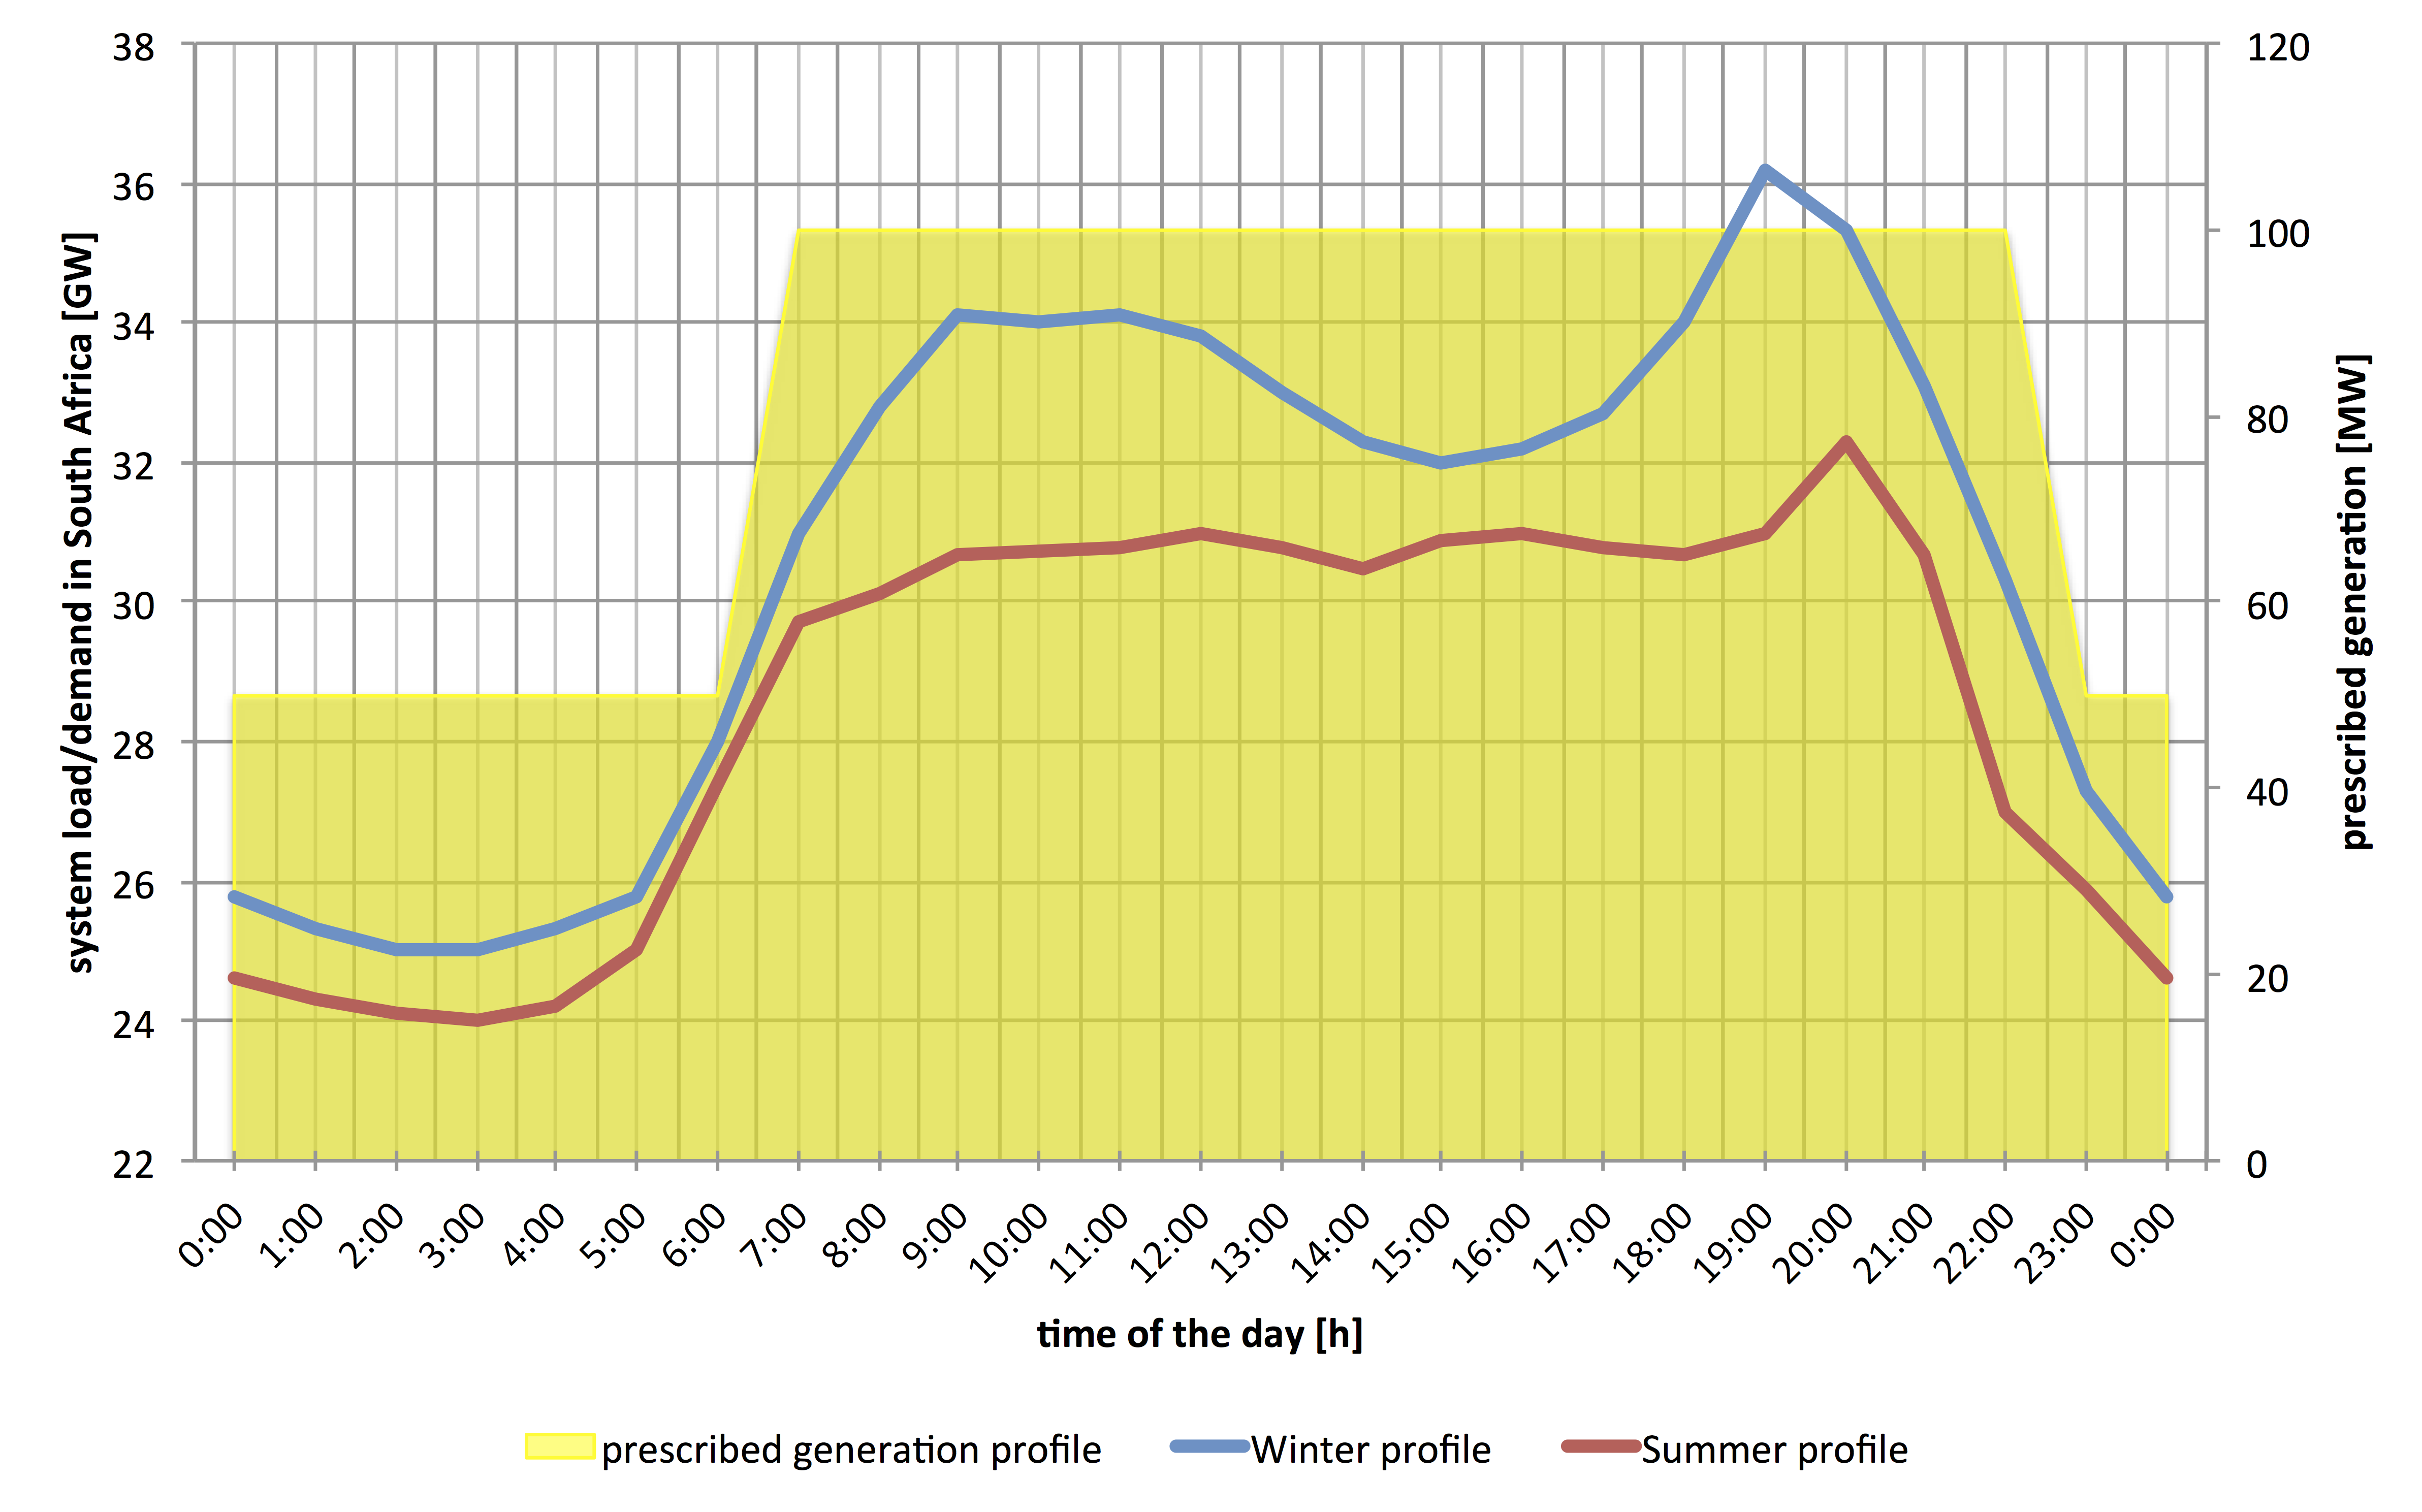
\includegraphics[width=1\linewidth]{FIG/LoadScenarios}
\caption[South Africa daily average system load/demand for summer and winter days, with scheduled power production curve.]{South Africa daily average system load/demand for summer and winter days, with scheduled power production curve.}\label{LoadScenarios}
\end{figure}
%For the comparison the power plants there system design is forced to cover 90~\% of the scheduled electricity production over the first year.  Usually, in feed-in contracts the power output is fixed at specified values. The overproduction is not content of these contracts and is not remunerated. In order to generate exploitable and comparable results and also considering the common feed-in contracts for power plants, the hourly power production is cut to the planed values. So overproduction will not considered in the evaluation and analyses of the systems.
In this comparison, the system design must handle 90~\% of the scheduled electricity production over the first year. Usually, in feed-in contracts, the deliverable energy is fixed. Any overproduction is not covered by such contracts and is not remunerated. In order to generate exploitable and comparable results and considering standard feed-in contracts, the hourly power production is cut to the planned values and thus overproduction is not considered in this analysis.

%The results of the simulated scenarios and the financial analyses will be rated in two selected categories:
The results of the simulation and the financial analyses will be evaluated by the following quantitative measures:
\begin{itemize}
%\item \textbf{Load curve covering factor} [\%]: The Load curve covering factor (LCCF) describes quantitative how effective the power plant follows the required load curve of the scenarios.
\item \textbf{Load curve covering factor} [\%]: The load curve covering factor (LCCF) is an effectiveness measure describing how closely the plant follows the load curve.
%\item \textbf{Levelized cost of electricity} [\textcent /kWh]: The levelized cost of electricity (LCOE) represents the total project lifecycle costs. It is the present value of project costs expressed in cents per kilo-hour of electricity generated by the system over its life. \cite{NREL2015a}
\item \textbf{Levelized cost of electricity} [\textcent /kWh]: The levelized cost of electricity (LCOE) represents the total project life-cycle costs. It is the present value of project costs expressed in cents per kilowatt-hour of electricity generated by the system over its life. \cite{NREL2015a}
\end{itemize}
%There is a huge difference between the mentioned LCCF and the widespread capacity factor (CF). The CF is the ratio of the system's predicted electrical output in the first year of operation to the nameplate output, which is equivalent to the quantity of energy the system would generate if it operated at its nameplate capacity for every hour of the year \cite{NREL2015a}. As it is mentioned above is the LCCF calculated from the sum value of load covering in each hour of the year.
There is an important difference between the LCCF and the widely-used \emph{capacity factor} (CF). The CF is the ratio of the system's electrical output in the first year of operation to the nameplate output, which is equivalent to the quantity of energy the system would generate if it operated at its nameplate capacity for every hour of the year \cite{NREL2015a}. The LCCF is calculated from the sum value of load coverage in each hour of the year.
%At a covering of 100~\% of the predicted load the solar power plants would produce \SI{711.75}{GWh} per year. But at a 100~\% CF the solar power plants would need to produce \SI{876.00}{GWh} per year. Therefore is in the selected scenario a maximum CF of just 81.25~\% with a full covering of the predicted load possible.
At a coverage of \SI{100}{\percent} of the predicted load, the solar power plants would produce \SI{711.75}{\giga\watt\hour\per\year}, but at a \SI{100}{\percent} CF they would need to produce \SI{876.00}{\giga\watt\hour\per\year}. In the current scenario, the maximum CF is just \SI{81.25}{\percent}, even though full load coverage is possible.


\subsection{Location and weather data} \label{Location and weather data}
%For the simulation of the solar power plants the locations and weather parameter of Upington, Northern Cape was used. This location is situated in a region with one of the highest irradiation values of the country, but also has a good water access by the Orange River. This locations was mentioned before in Chapter~\ref{Solar power in South Africa} and is marked in the GHI- and DNI-maps of SA in Figure \ref{irradiation} on Page \pageref{irradiation}.
In this simulation, locations and weather data for Upington, Northern Cape were used. This region has among the highest irradiation values in the country, but also has good water access due to the Orange River. This location was mentioned before in Chapter~\ref{Solar power in South Africa} and is marked in the GHI- and DNI-maps of SA in Figure \ref{irradiation} on page \pageref{irradiation}. 
 
\begin{table}[!h]  
  \centering
	\begin{tabular}{  p{4.0cm}  C{4.0cm}  C{3.0cm} } 

	\hline	
\textbf{Item}  & \textbf{Value} & \textbf{Unit} \\ \hline \hline
Location & Upington & -\\ 
Station ID &  684240& -  \\ 
Data source & White Box Technologies, Inc. (31.05.2015) & -\\ \hline
Latitude & -28.40 &$\,^{\circ}$N \\ 
Longitude &  21.27 &$\,^{\circ}$E \\ 
Elevation &  836 & m \\ 
Total GHI per year  &  2~280 & \si{\kilo\watt\hour\per\square\metre}\\ 
Total DNI per year &  2~621 & \si{\kilo\watt\hour\per\square\metre}\\ 
Total DHI per year &  516 & \si{\kilo\watt\hour\per\square\metre}\\ 
Mean temp. &  21 & \si{\celsius}\\ 
Mean wind speed & 3.3 & \si{\metre\per\second}\\ \hline
\end{tabular}
\caption[Location and characteristics for the simulation in SAM.]{Location and characteristics for the simulation in SAM.}\label{tbl: Location}
\end{table}


%The input weather data for the simulation with SAM are in the EPW-format (EnergyPlus Weather Data) and produced by White Box Technologies, Inc. \cite{WhiteBoxTechnologies2015}. The EPW-files are data sets of hourly values of solar radiation and meteorological elements for a typical one-year period. This includes air temperature, dew point temperature, relative Humidity, atmospheric pressure, global horizontal solar radiation, diffuse Horizontal solar radiation, direct normal radiation, wind Speed, wind Direction and cloud cover. The for the simulation most relevant values are summarized in Table \ref{tbl: Location}. The hourly values of global horizontal and direct normal irradiance from the EPW-file is shown in Figure~\ref{Upington_GHI/DNI}. The highest irradiance value during the summer time is 1~\SI{199}{Wh/m}^2 for GHI and 1~\SI{154}{Wh/m}^2 for DNI. At the shortest day the highest irradiance is \SI{625}{Wh/m}^2 for GHI and \SI{820}{Wh/m}^2 for DNI.
The weather data for the simulation in SAM are in EPW format (EnergyPlus Weather Data) and produced by White Box Technologies, Inc. \cite{WhiteBoxTechnologies2015}. The EPW files are data sets of hourly values of solar radiation and meteorological elements for a typical one-year period. These include air temperature, dew point temperature, relative humidity, atmospheric pressure, global horizontal solar radiation, diffuse horizontal solar radiation, direct normal radiation, wind speed, wind direction and cloud cover. The most relevant parameters for this simulation are summarized in Table \ref{tbl: Location}. The hourly values of global horizontal and direct normal irradiance from the EPW file are shown in Figure~\ref{Upington_GHI/DNI}. The highest irradiance value during the summer is \SI{1199}{\watt\hour\per\square\metre} for GHI and \SI{1154}{\watt\hour\per\square\metre} for DNI. At the northern solstice, the highest irradiance is \SI{625}{\watt\hour\per\square\metre} for GHI and \SI{820}{\watt\hour\per\square\metre} for DNI.


\begin{figure}[!htbp]
        \centering
                \begin{subfigure}[b]{1\textwidth}
                \centering
                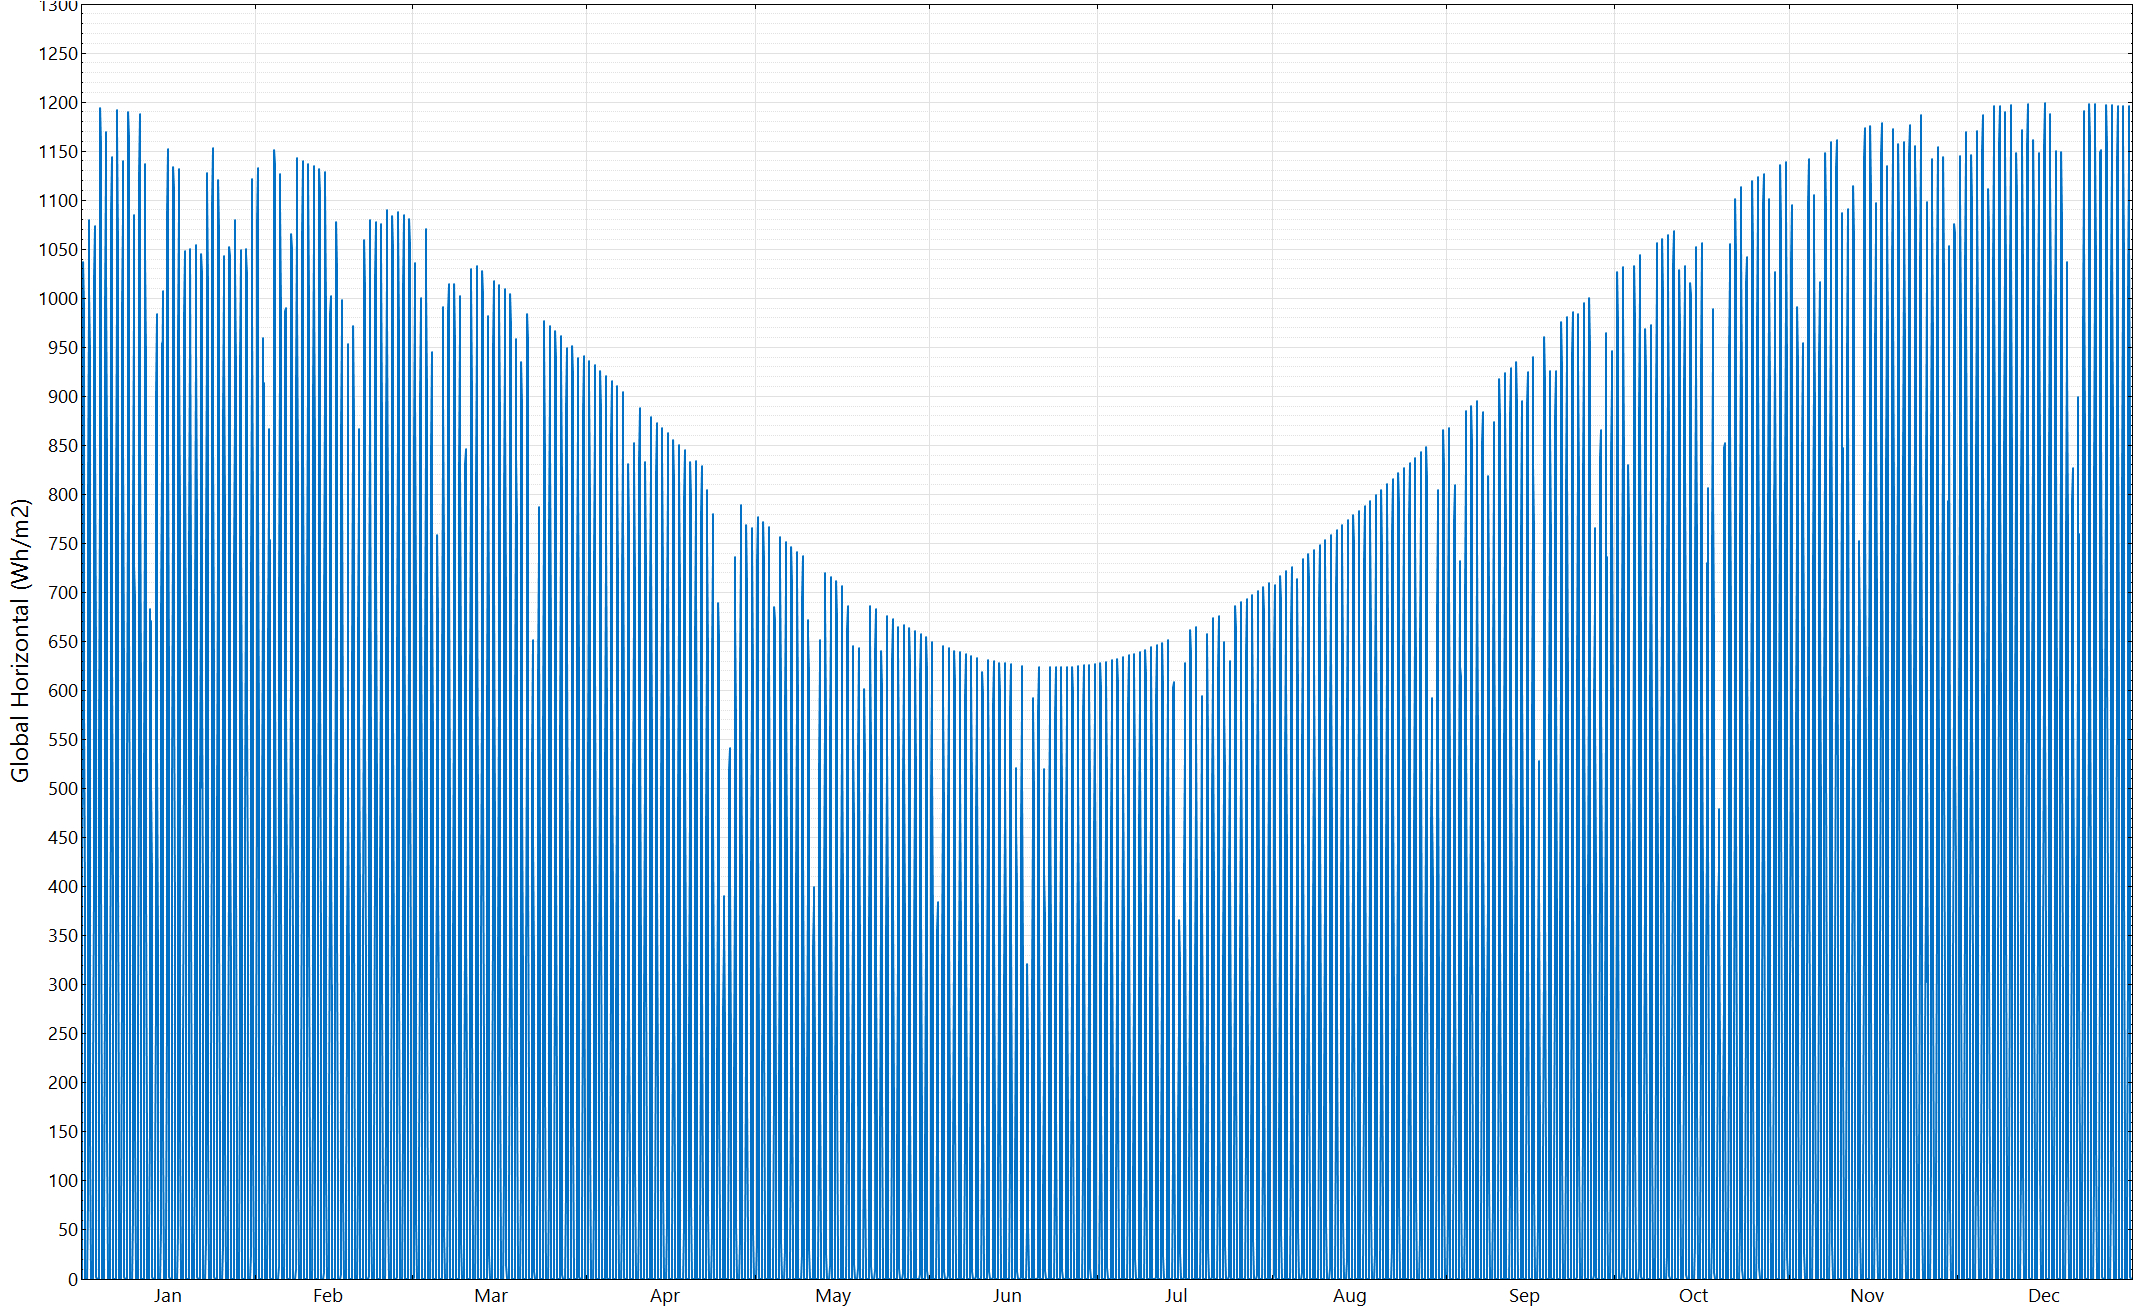
\includegraphics[width=1\textwidth]{FIG/Upington_GHI}
                \caption{Global horizontal}\label{Upington_GHI}
        \end{subfigure}%
\par\medskip % Linebreak      
        \begin{subfigure}[b]{1\textwidth}
                \centering
                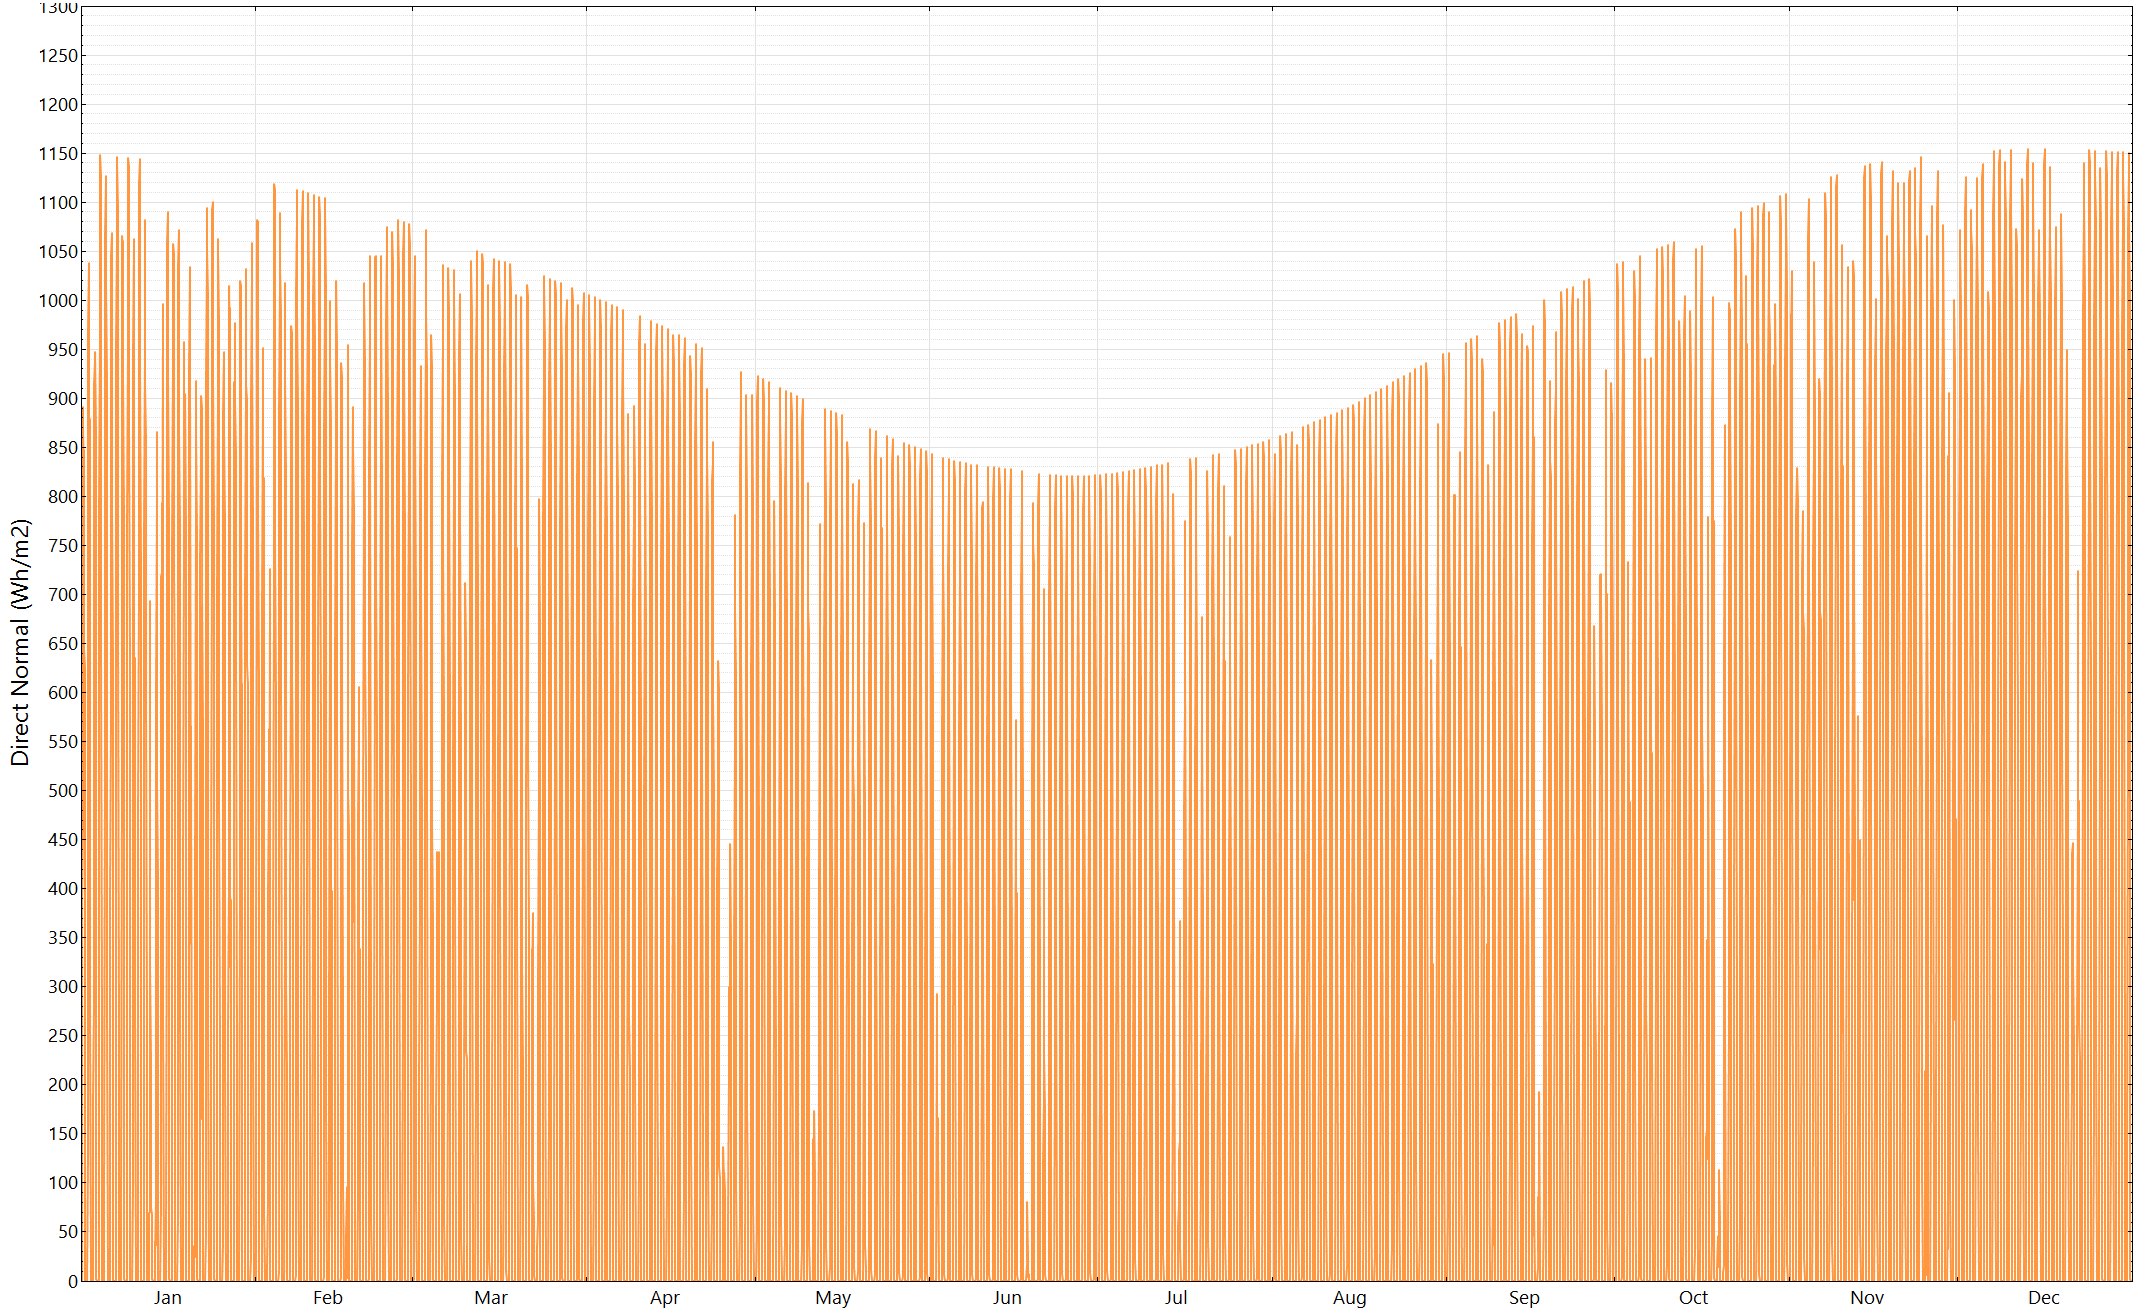
\includegraphics[width=1\textwidth]{FIG/Upington_DNI}
                \caption{Direct normal }\label{Upington_DNI}
        \end{subfigure}%

        \caption[Hourly values of irradiance over a full year from Upington used in the simulation.]{Hourly values of irradiance over a full year from Upington used in the simulation.}\label{Upington_GHI/DNI}
\end{figure}
\newpage \noindent
%Most relevant for the simulation is also the position of the sun. SAM calculates the path of the sun by the position of longitude and latitude. Figure~\ref{SunPathUpington} shows the sun path diagram of Upington. From this it appears that the longest day in Upington has \SI{13}{h} and \SI{56}{minutes} with a maximum sun height of 85.05$\,^{\circ}$ while the shortest day has just \SI{10}{h} and \SI{19}{minutes} and a maximum sun height of 35.93$\,^{\circ}$.
SAM calculates the path of the sun by the position of longitude and latitude. Figure~\ref{SunPathUpington} shows the solar path diagram at Upington. The longest day in Upington has a duration of \SI{13}{h} and \SI{56}{minutes} with a maximum sun height of \SI{85.05}{\degree} while the shortest day has a duration of just \SI{10}{h} and \SI{19}{minutes} and a maximum sun height of \SI{35.93}{\degree}.

\begin{figure}[htbp]  
\centering
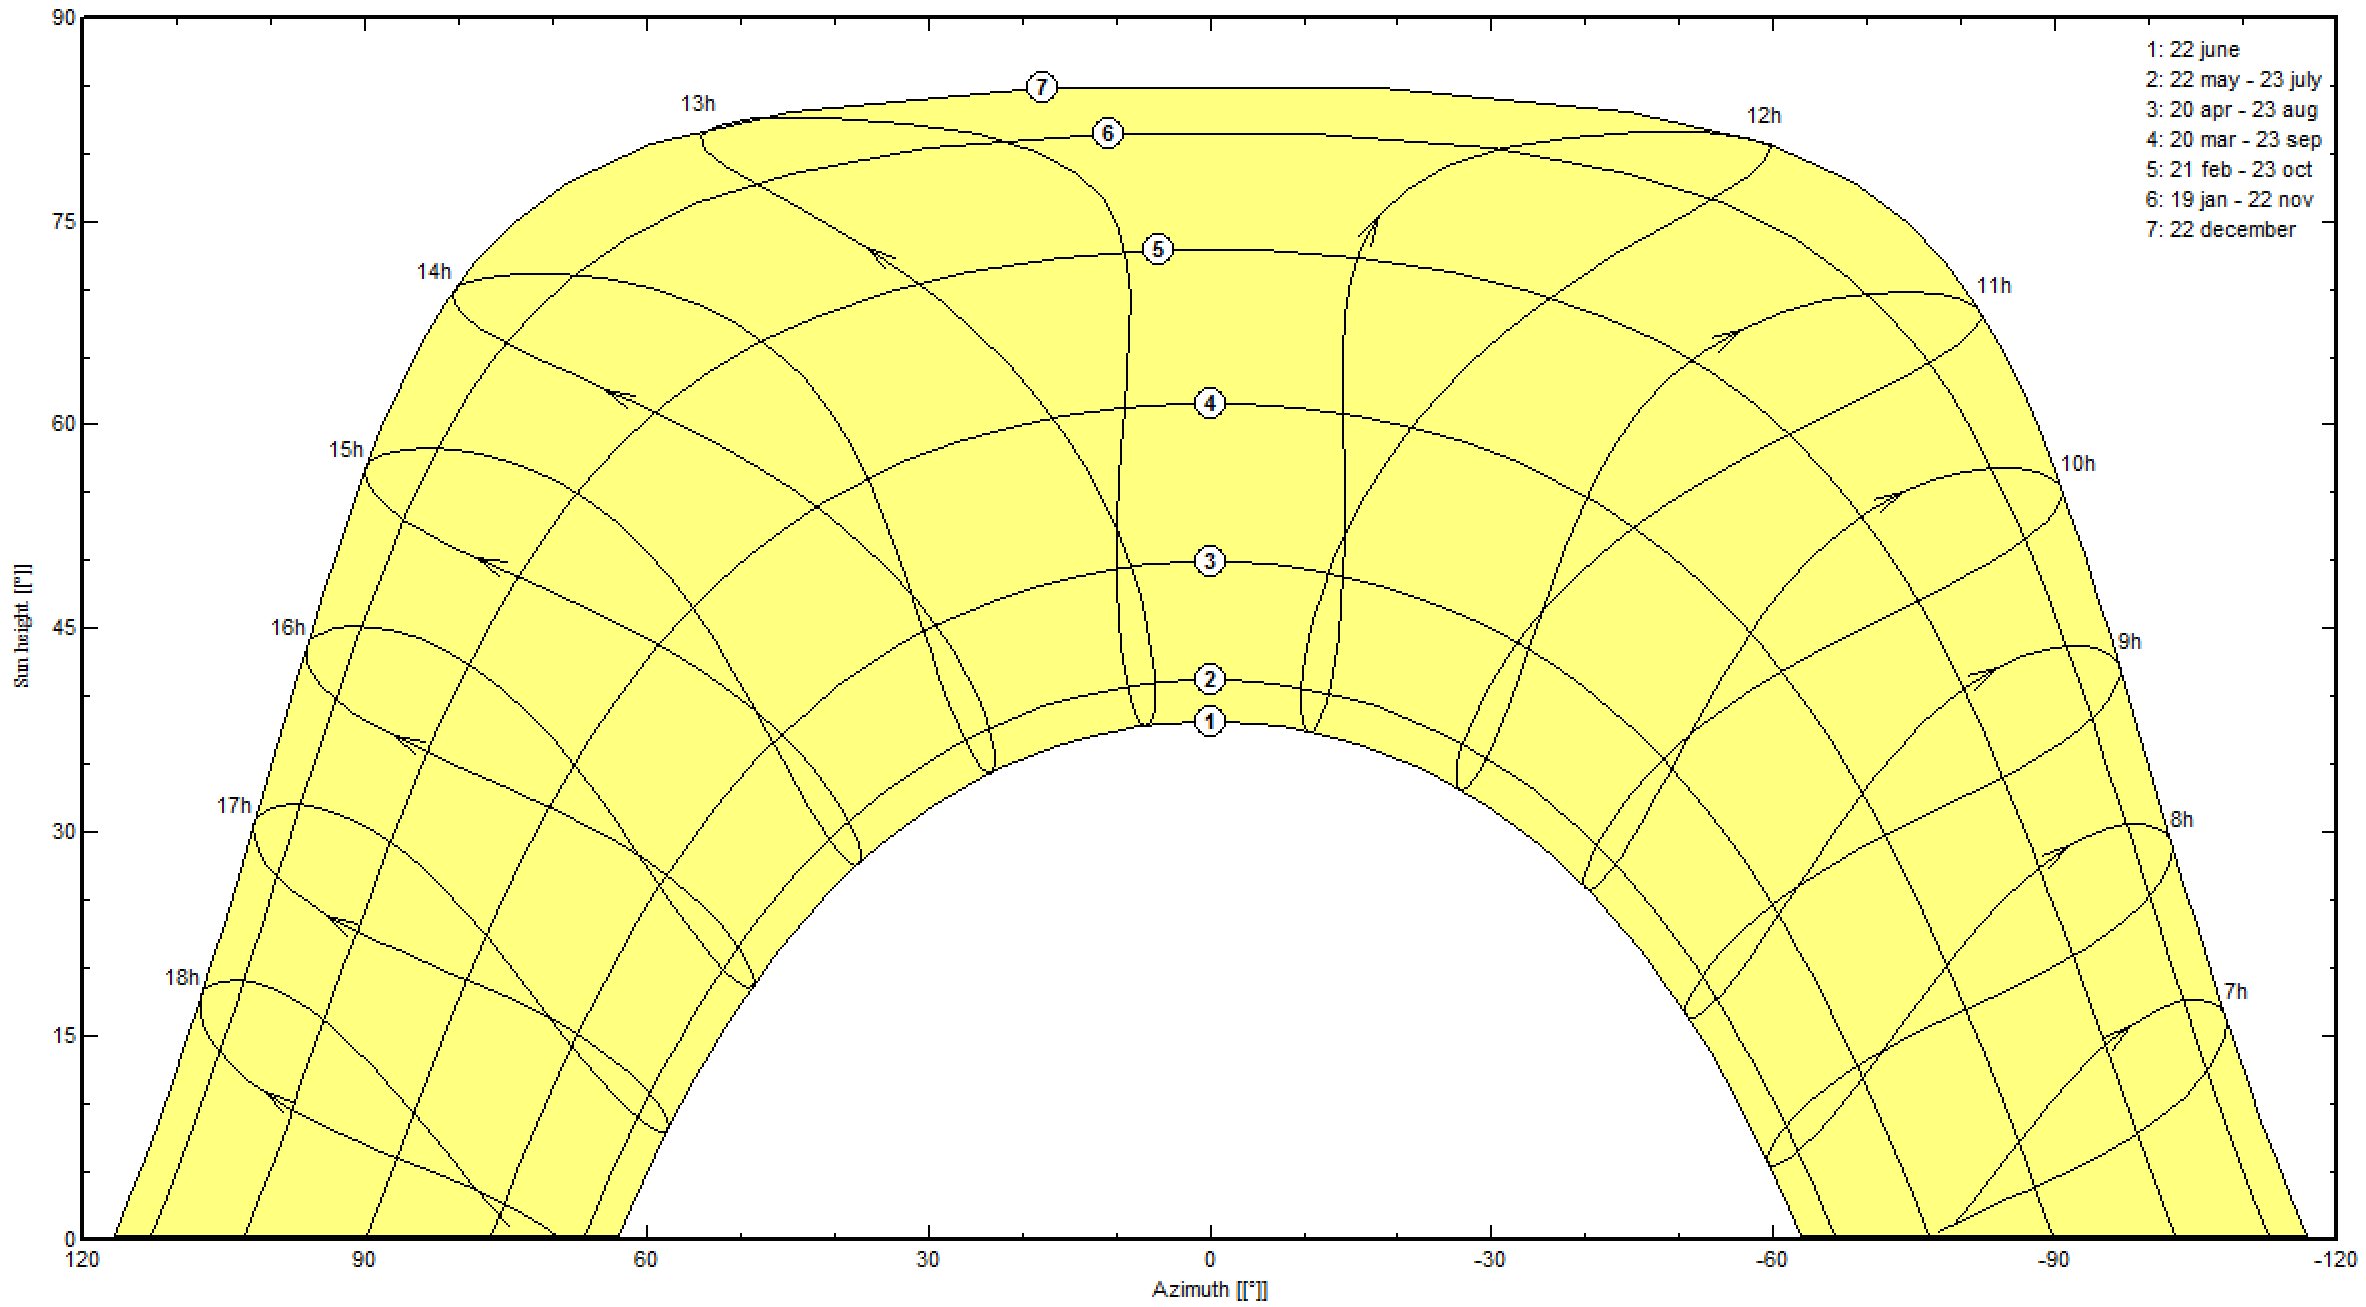
\includegraphics[width=0.95\linewidth]{FIG/SunPathUpington}
\caption[Solar path diagram for Upington.]{Solar path diagram Upington \cite{PVsystSA2015}.}\label{SunPathUpington}
\end{figure}
\pagebreak 
